% \documentclass[letterpaper,12pt]{report}
% \usepackage[pdftex]{graphicx}
% \usepackage[spanish]{babel}
% \usepackage[latin1]{inputenc}
% \pagestyle{plain}

% \begin{document}
% \addtolength{\hoffset}{-0.5cm}
% \addtolength{\textwidth}{1cm}
% \addtolength{\textheight}{1cm}
% \chapter{UML}

%%%%%%%%%%%%%%%%%%%%%%%%%% CLASE Apriori%%%%%%%%%%%%%%%%%%%%%%%%%%%%%%%%%%%%%%%%%%%%
\begin{figure}
\section{Dise\~no}
\subsection{Diagramas de Colaboraci\'on}
\subsubsection{Clase Apriori}
\centering
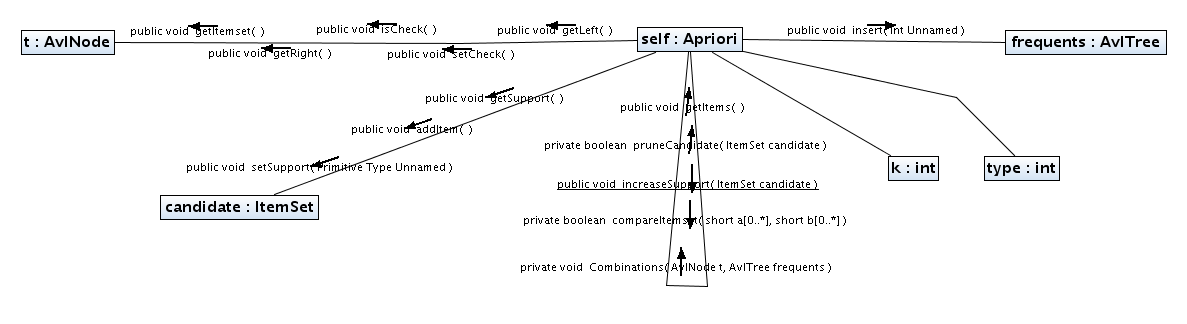
\includegraphics[angle=90, width=0.33\textwidth]{imgsColaboracion/Apriori/Combinations.png}
\caption{Combinations}
\end{figure}
\newpage
\begin{figure}
\centering
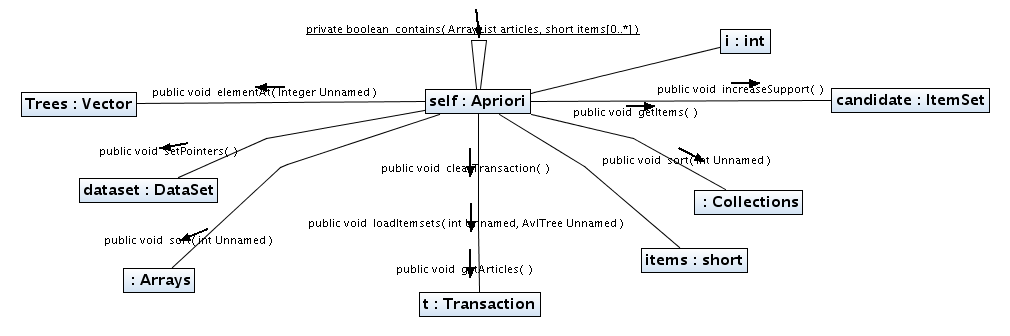
\includegraphics[angle=90, width=0.41\textwidth]{imgsColaboracion/Apriori/IncreaseSuport.png}
\caption{IncreaseSuport}
\end{figure}
\newpage
\begin{figure}
\centering
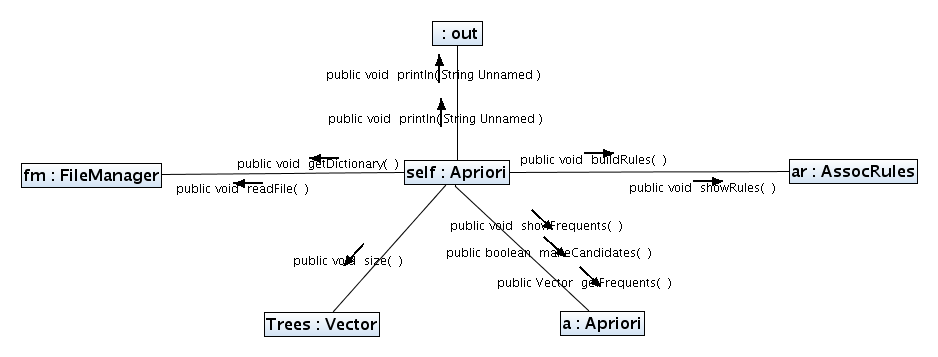
\includegraphics[angle=90, width=0.47\textwidth]{imgsColaboracion/Apriori/main.png}
\caption{main}
\end{figure}
\newpage
\begin{figure}
\centering
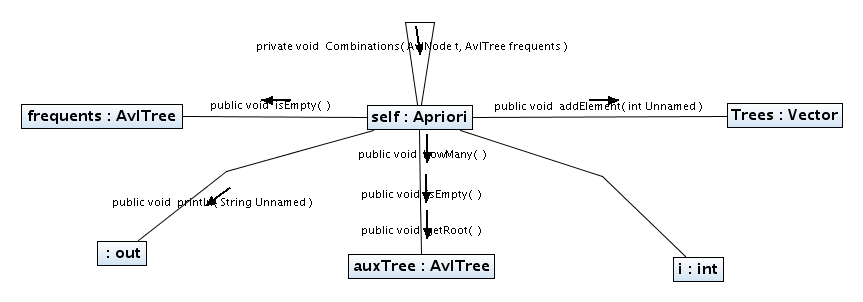
\includegraphics[angle=90, width=0.43\textwidth]{imgsColaboracion/Apriori/makeCandidates.png}
\caption{makeCandidates}
\end{figure}
\newpage
\begin{figure}
\centering
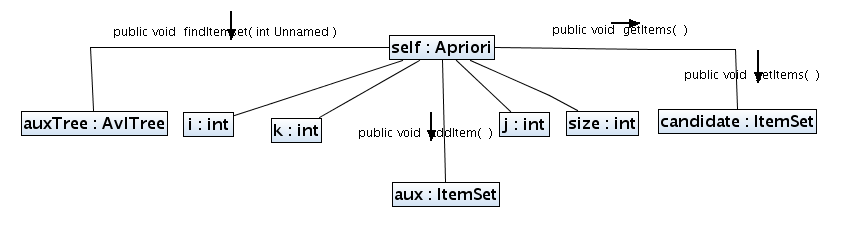
\includegraphics[angle=90, width=0.33\textwidth]{imgsColaboracion/Apriori/pruneCandidate.png}
\caption{pruneCandidate}
\end{figure}
\newpage
%%%%%%%%%%%%%%%%%%%%%%%%%% CLASE  EuipAsso%%%%%%%%%%%%%%%%%%%%%%%%%%%%%%%%%%%%%%%%%%%%
\begin{figure}
\subsubsection{Clase EuipAsso}
\centering
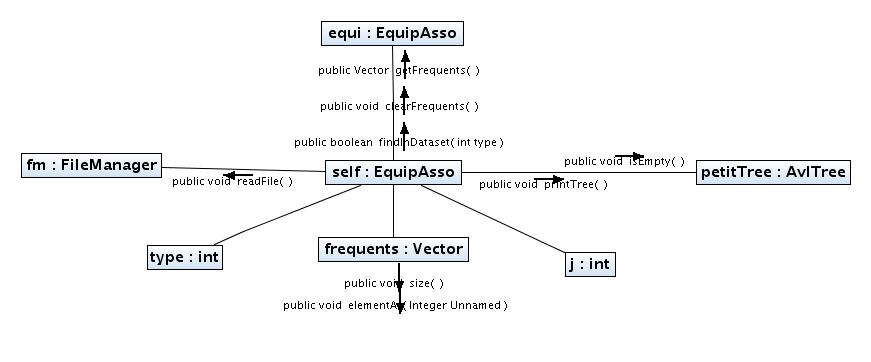
\includegraphics[width=1.2\textwidth]{imgsColaboracion/EuipAsso/EquipAsso/main.png}
\caption{main}
\end{figure}
\newpage
\begin{figure}
\centering
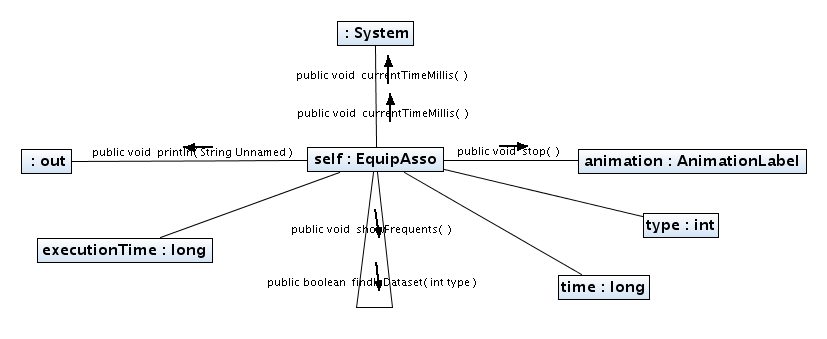
\includegraphics[width=1.2\textwidth]{imgsColaboracion/EuipAsso/EquipAsso/run.png}
\caption{run}
\end{figure}
\newpage
\begin{figure}
\centering
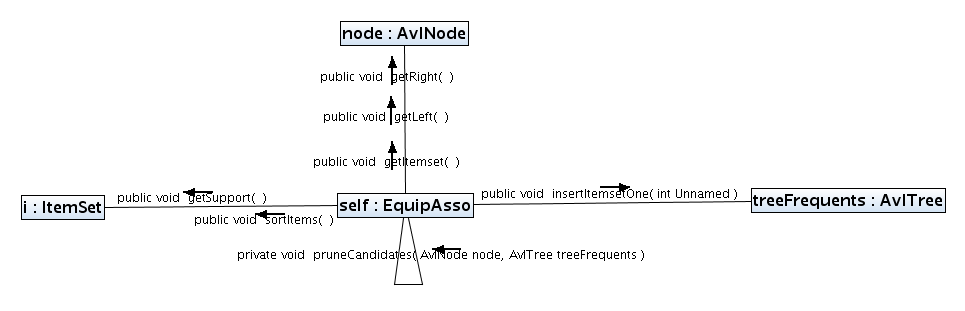
\includegraphics[angle=90,width=0.4\textwidth]{imgsColaboracion/EuipAsso/EquipAsso/pruneCandidates.png}
\caption{pruneCandidates}
\end{figure}
\newpage
%%%%%%%%%%%%%%%%%%%%%%%%%% CLASE  Combinations%%%%%%%%%%%%%%%%%%%%%%%%%%%%%%%%%%%%%%%%%%%%
\begin{figure}
\subsubsection{Clase Combinations}
\centering
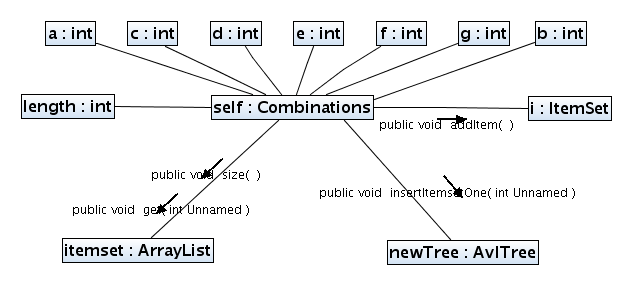
\includegraphics[width=1\textwidth]{imgsColaboracion/EuipAsso/Combinations/combine7.png}
\caption{combine7}
\end{figure}
\newpage
\begin{figure}
\centering
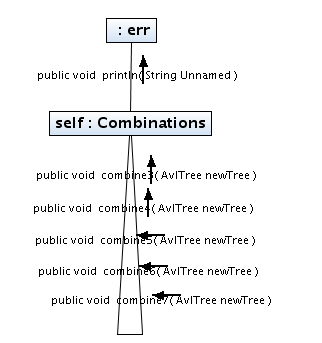
\includegraphics[width=0.6\textwidth]{imgsColaboracion/EuipAsso/Combinations/letsCombine.png}
\caption{letsCombine.png}
\end{figure}
\newpage
%%%%%%%%%%%%%%%%%%%%%%%%%% CLASE  BaseConditionals %%%%%%%%%%%%%%%%%%%%%%%%%%%%%%%%%%%%%%%%%%%%
\begin{figure}
\subsubsection{Clase BaseConditionals}
\centering
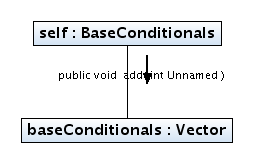
\includegraphics[width=0.3\textwidth]{imgsColaboracion/FPGrowth/BaseConditionals/addBaseConditionals.png}
\caption{addBaseConditionals}
\end{figure}
\newpage
\begin{figure}
\centering
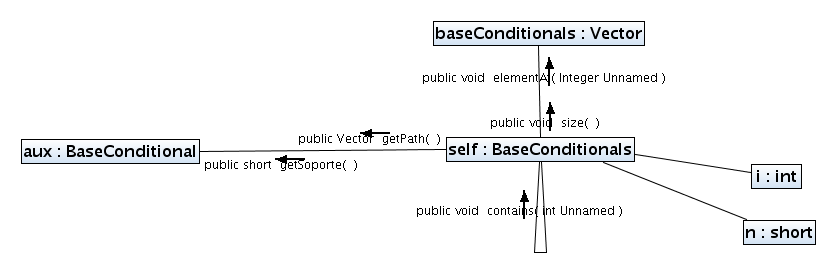
\includegraphics[angle=90,width=0.3\textwidth]{imgsColaboracion/FPGrowth/BaseConditionals/findItem.png}
\caption{findItem}
\end{figure}
\newpage
%%%%%%%%%%%%%%%%%%%%%%%%%% CLASE  Combinations %%%%%%%%%%%%%%%%%%%%%%%%%%%%%%%%%%%%%%%%%%%%
\begin{figure}
\subsubsection{Clase Combinations}
\centering
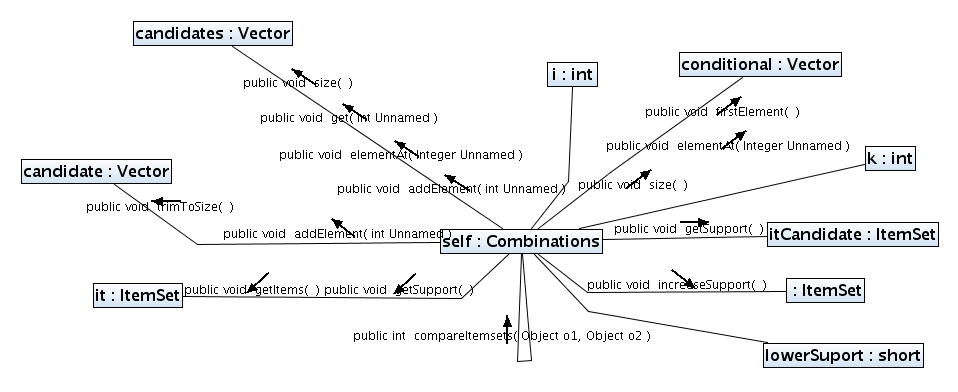
\includegraphics[angle=90,width=0.5\textwidth]{imgsColaboracion/FPGrowth/Combinations/addCandidates.png}
\caption{addCandidates}
\end{figure}
\newpage
\begin{figure}
\centering
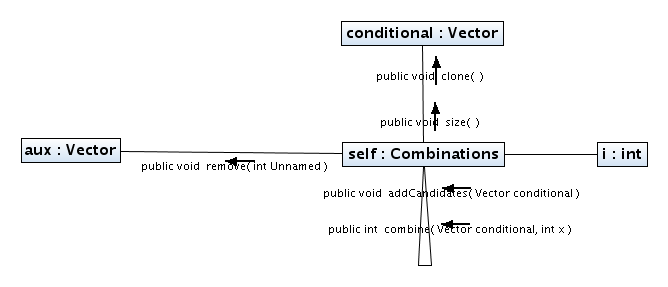
\includegraphics[angle=90,width=0.5\textwidth]{imgsColaboracion/FPGrowth/Combinations/Combine.png}
\caption{Combine}
\end{figure}
\newpage
%%%%%%%%%%%%%%%%%%%%%%%%%% CLASE  FPGrowth %%%%%%%%%%%%%%%%%%%%%%%%%%%%%%%%%%%%%%%%%%%%
\begin{figure}
\subsubsection{Clase FPGrowth}
\centering
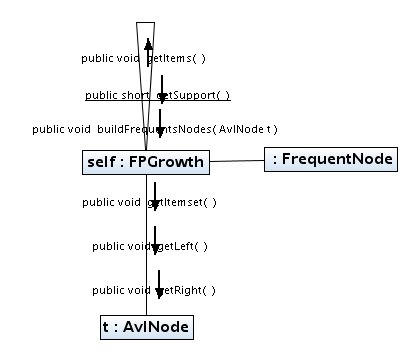
\includegraphics[width=0.8\textwidth]{imgsColaboracion/FPGrowth/FPGrowth/builtFrecuenceNode.png}
\caption{builtFrecuenceNode}
\end{figure}
\newpage
\begin{figure}
\centering
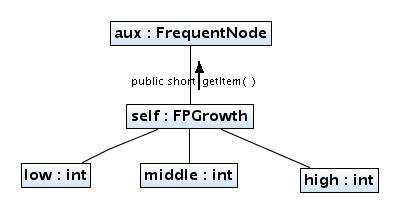
\includegraphics[width=0.7\textwidth]{imgsColaboracion/FPGrowth/FPGrowth/FrequentNode.png}
\caption{FrequentNode}
\end{figure}
\newpage
%%%%%%%%%%%%%%%%%%%%%%%%%% CLASE  AvlTree %%%%%%%%%%%%%%%%%%%%%%%%%%%%%%%%%%%%%%%%%%%%
\begin{figure}
\subsubsection{Clase AvlTree}
\centering
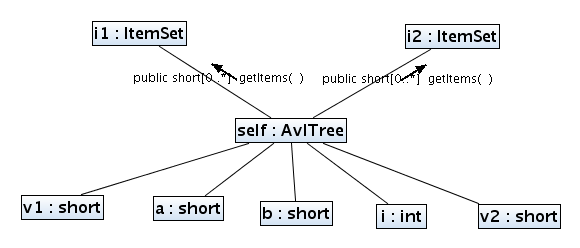
\includegraphics[width=0.9\textwidth]{imgsColaboracion/Utils/AvlTree/compareItems.png}
\caption{compareItems}
\end{figure}
\newpage
\begin{figure}
\centering
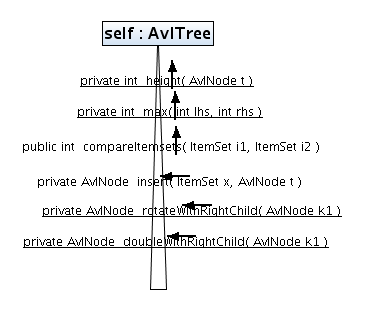
\includegraphics[width=0.7\textwidth]{imgsColaboracion/Utils/AvlTree/insert.png}
\caption{insert}
\end{figure}
\newpage

%%%%%%%%%%%%%%%%%%%%%%%%%% CLASE  DataSet %%%%%%%%%%%%%%%%%%%%%%%%%%%%%%%%%%%%%%%%%%%%
% \subsubsection{Clase DataSet}
% \begin{figure}
% \centering
% 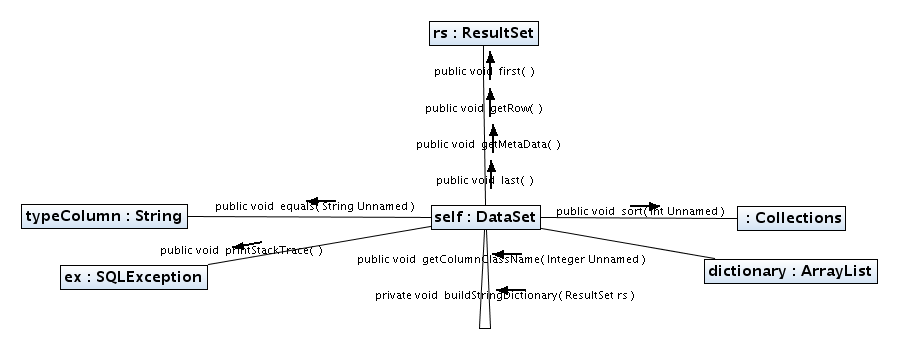
\includegraphics[angle=90,width=0.49\textwidth]{imgsColaboracion/Utils/DataSet/builtDictionary.png}
% \caption{builtDictionary}
% \end{figure}
% \newpage
% \begin{figure}
% \centering
% 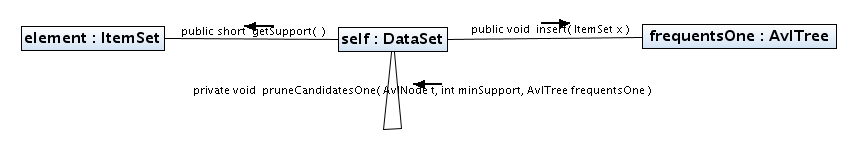
\includegraphics[width=1.2\textwidth]{imgsColaboracion/Utils/DataSet/pruneCandidatesOne.png}
% \caption{pruneCandidatesOne}
% \end{figure}
% \newpage
% \begin{figure}
% \centering
% 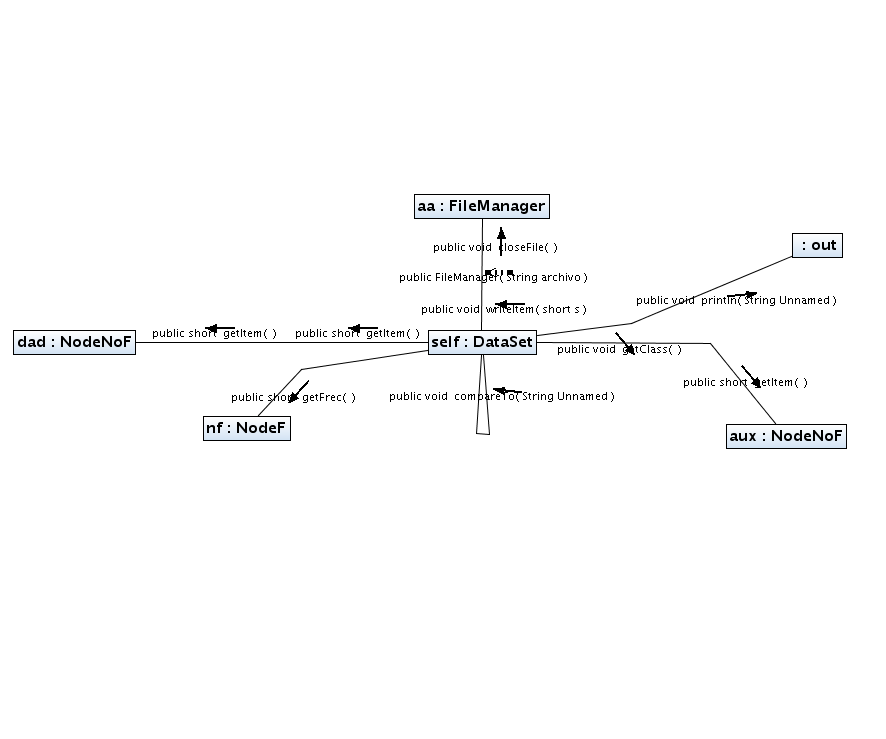
\includegraphics[width=1.2\textwidth]{imgsColaboracion/Utils/DataSet/saveTree.png}
% \caption{saveTree}
% \end{figure}
% \newpage
%%%%%%%%%%%%%%%%%%%%%%%%%% CLASE  Transaction %%%%%%%%%%%%%%%%%%%%%%%%%%%%%%%%%%%%%%%%%%%%
% \begin{figure}
% \subsubsection{Clase Transaction}
% \centering
% 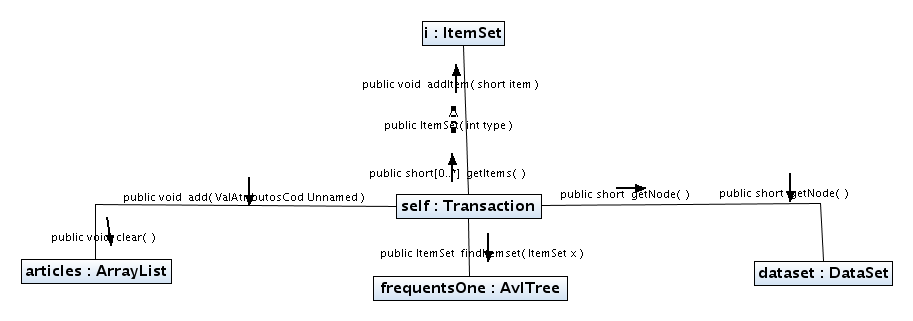
\includegraphics[width=1.2\textwidth]{imgsColaboracion/Utils/Transaction/loadItems.png}
% \caption{loadItems}
% \end{figure}
% \newpage
% 
% \begin{figure}
% \centering
% 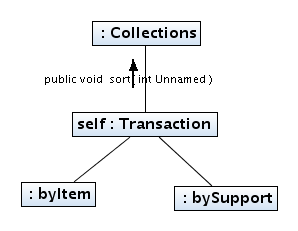
\includegraphics[width=0.4\textwidth]{imgsColaboracion/Utils/Transaction/sortBySupport.png}
% \caption{sortBySupport}
% \end{figure}


% \end{document}
